\documentclass[a4paper,11pt,pdf]{pacmanreport}

\usepackage{helvet}
\usepackage{graphicx}

%%=== Aditional packages
\usepackage{hyperref} % references
\usepackage{amssymb}
\usepackage{tikz}

\usetikzlibrary{shapes,arrows}
\usepackage{mathtools}
\usepackage{float}
\usepackage{subcaption}

%%=====================


\graphicspath{{images/}{../shared_images/}}

%% ================================
%% PROJECT INFO 

\project{}
\projectid{FP7-IST-60918}
\projectstart{1 March 2013}
\duration{36}

%% ================================
%% MILESTONE INFO 

\title{Reactive haptic exploration control strategies ready for integration with planning}
\deliverableid{Milestone 4.2}
\author{Manuel Bonilla, Carlos Rosales, Federico Spinelli, Marco Gabiccini}
% \author{Carlos Rosales, Federico Spinelli, Manuel Bonilla, Marco Gabiccini}
\address{Centro di Ricerca ``E. Piaggio'', Universit\`{a} di Pisa}
% \email{carlos.rosales@for.unipi.it}
\email{manuel.bonilla@centropiaggio.unipi.t}
\headertitle{Exploration strategies}
% \headerauthor{C. Rosales, F. Spinelli, M. Bonilla, M. Gabiccini}
\headerauthor{M. Bonilla, C. Rosales, F. Spinelli, M. Gabiccini}
\duedate{2015-02-28}
\submissiondate{2014-02-28}
\leadpartner{Universit\`{a} di Pisa}
\revision{draft}
\disseminationlevel{PU}


%% UNCOMMENT: to get the logo; if you've copied this file to a directory yearX/wpY/ then this should work
\reportlogo{pacmanlogo.png}

%% ======= Defining tikz style
\tikzstyle{block} = [draw, fill=blue!5, rectangle, 
    minimum height=3em, minimum width=6em]
\tikzstyle{block_small} = [draw, fill=blue!5, rectangle, 
    minimum height=3em, minimum width=3em]
\tikzstyle{sum} = [draw, fill=blue!5, circle]
\tikzstyle{intersection} = [fill,circle,minimum size=3pt,inner sep=0pt]
\tikzstyle{input} = [coordinate]
\tikzstyle{output} = [coordinate]
%%==============


\begin{document}

\maketitle

\begin{abstract}
\noindent In  this milestone 
\end{abstract}


\vspace{.2em}
\hrule

\vspace{.2em}
\footnotesize

\tableofcontents

\normalsize

\newpage

% \section{Milestone Summary and Context}

% What was the milestone that you are examining? What were the criteria for achieving it? What role does achievement of the milestone play in the whole project? How will its achievement as presented in this report contribute to the PaCMan scenarios and prototypes? 


% \newpage

% \section{Report on Milestone Achievement}

% How have the tasks been addressed? To what extent have the intended objectives been achieved? Why, how -- or why not? In particular what concrete acceptance tests, or experimental results show that the milestone has been achieved.


% \section{Annexes}

% Here you should briefly describe the papers attached that provide evidence for achievement of the milestone. Mention titles, authors, publication info; abstract; and a one-liner relating the publication back to the discussion on actual work performed. 



%!TEX root = MS42.tex
%\section{Introduction}

In recent years, there has been growing interest in the development of a standardized framework for robotic implementations, where the robots interdisciplinary code and software could be easy to write and accessible to everyone. This is the philosophy of the \textit{Robot Operating System} (\textbf{ROS}), a flexible framework which provides all the instruments to develop and build robust and robot-independent applications, allowing researchers from different fields of robotics to share each others works with the great result of spreading the know-how.

Since ROS is the software framework used in PaCMan we developed a hardware interface for the robots used in the experimental platforms. However, this interface is just useful to command the robot using torque references. There are different strategies to generate the torque references to move a robot manipulator, they are designed for different situation for example under uncertainty, which main problem faced in PaCMan Project, in this case in the robot dynamics. Other strategies to deal with multiple goal references at kinematic and dynamic level were also implemented.

% \subsection{Project Goals}

% The aim of this milestone report is focused on the development of a ROS-enabled software environment for controlling the manipulator KUKA LWR IV, used in the PaCMan platforms. 

After a first phase of studying and analyzing some of the novel approaches for robot control, the default control strategies provided by the manufacturer has been extended, implementing a new set of controllers. 
The development of the controllers, including tuning and debugging, has been realized with the support of \textit{Gazebo}, a high performance realistic simulator which, interacting with ROS, gives the opportunity to test the efficiency of user-implemented control algorithms. 

Finally, the last phase consisted in pursuing experiments to test the implemented control strategies on the physical robot, arising a variety of practical issues which don't come out in simulation, that are explained in detail in this document.

\newpage

\subsection{Kuka LWR4+}
\label{sec:kuka}

The KUKA Lightweight Robot IV shown in Fig.~\ref{fig:kuka_arm} is a 7-axis industrial manipulator which finds a wide employment in robotic research due to its flexibility and modularity.
%, including a payload capacity of 7 Kg. 
%In addition, the seventh axis makes the robot redundant, which mean that, for a given position and orientation of the end effector, there exist multiple configurations in the joints space. 
Each joint is equipped with a position and a torque sensor, which allow the robot to be regulated using position, velocity and torque commands.
\begin{figure}
\centering
\includegraphics[width=0.4\textwidth]{kuka}
\caption{KUKA Lightweight Robot IV.}
\label{fig:kuka_arm}
\end{figure}

\subsubsection{Hardware interface}
The robot provides three different control strategies as default setting, which are described below~\cite{kukafri}.

\paragraph{Position Controller}
Desired joint positions are regulated through the use of an internal \textit{PID} as
\begin{equation}
\mathbf{q}_{LBR} = \mathbf{q}_{FRI},
\label{eq:positioncontroller}
\end{equation}
where $\mathbf{q}_{FRI}$ is the commanded joint positions.

\paragraph{Cartesian Stiffness Controller}
The Cartesian stiffness controller is characterized by the following control law:
\begin{equation}
\tau_{cmd} = J^T(k_c(x_{FRI} - x_{msr}) + F_{FRI}) + D(d_c) + f_{dynamics}(q,\dot{q},\ddot{q})
\label{eq:cartesianstiffnesscontroller}
\end{equation}
where $\tau_{cmd}\in\mathbb{R}^7$ is the  control torque, $x_{FRI}\in\mathbb{R}^{12}$ is the commanded cartesian position, $x_{msr}\in\mathbb{R}^{12}$ is the measured cartesian position, $k_c\in\mathbb{R}^{7\times 7}$is the commanded cartesian stiffness, $D(d_c)\in\mathbb{R}^7$ is the commanded damping term, $F_{FRI}\in\mathbb{R}^6$ is the commanded cartesian force, and $f_{dynamics}(q,\dot{q},\ddot{q})\in\mathbb{R}^7$ is the gravity compensation term.

\paragraph{Axis-specific Stiffness Controller}
The axis-specific stiffness controller is similar to the cartesian stiffness controller, but it takes commands in joints space:
\begin{equation}
\tau_{cmd} = k_j(q_{FRI} - q_{msr}) + D(d_j) + \tau_{FRI} + f_{dynamics}(q,\dot{q},\ddot{q})
\label{eq:axisspecificstiffnesscontroller}
\end{equation}
where $\tau_{cmd}\in \mathbb{R}^7$ is the control torque, $q_{FRI}\in\mathbb{R}^7$ is the commanded joint position (reference position of a torsional spring), $q_{msr}\in\mathbb{R}^7$is the measured joint positions, $k_j\in\mathbb{R}^{7\times 7}$ is the commanded joint stiffnesses, $D(d_j)\in\mathbb{R}^7$ is the commanded damping term, $\tau_{FRI}\in\mathbb{R}^7$ is the added the joint effort, and $f_{dynamics}(q,\dot{q},\ddot{q})\in\mathbb{R}^7$ is the gravity compensation as before.

It is worth noting that, $f_{dynamics}(q,\dot{q},\ddot{q})\in\mathbb{R}^7$ is actually $f_{dynamics}(q)\in\mathbb{R}^7$ in all cases.

As seen in Fig.~\ref{fig:rosgazebointeraction}, there are two hardware interfaces developed for the Kuka LWR IV, that is, one that connects to the simulated and one that connects to the real robot, respectively. We decided to use the Axis-specific Stiffness Controller described above as the default strategy since it provides the more general setup. To this end, position and effort commands are possible using the same interface. The real hardware interface uses the \textit{Fast Research Interface} (FRI), a real-time proprietary software interface provided by Kuka able to read and write system variables of the robot and execute user-programs. The simulated hardware interface implements the Axis-specific Stiffness Controller, where it adds~$f_{dynamics}$ computed from the URDF model of the robot and the current joint values measured from the simulation. This way, any controller can switch between real and simulated hardware with very low extra effort.

%%%%%%%%%%%%%%%%%%%%%%%%%%%%%%%%%%%%%%%%%%%%%%%%%%%%%%%%%%%%%%%%%%%%%
%%%%%%%%%%%%%%%%%%%%%%%%%%%%%%%%%%%%%%%%%%%%%%%%%%%%%%%%%%%%%%%%%%%%%
%%%%%%%%%%%%%%%%%%%%%%%%%%%%%%%%%%%%%%%%%%%%%%%%%%%%%%%%%%%%%%%%%%%%%
\subsubsection{Implemented Controllers}\nocite{siciliano09}\nocite{bicchi13}
Exploiting the force $\tau_{FRI}$ in \eqref{eq:axisspecificstiffnesscontroller} (which will be the control strategy used for this project's purpose) as external torque command, a new set of ROS-enabled controllers has been developed in \textit{C++} language\footnote{Source code available at \url{https://github.com/CentroEPiaggio/kuka-lwr}}, following some interesting paradigms available in the robotics literature.

%\subsection{Robot Control Problem Definition}
Consider the expression of the dynamics of a $n$-links robot manipulator
\begin{equation}
M(q)\ddot{q} + C(q,\dot{q})\dot{q} + g(q) = \tau,
\label{eq:robotdynamics}
\end{equation}
where $M\in\mathbb{R}^{n \times n}$ is the manipulator inertia matrix, $C\in\mathbb{R}^{n \times n}$ the Coriolis and centripetal forces matrix, $g\in\mathbb{R}^n$ is the gravity forces vector, $q\in\mathbb{R}^n$ is the set of configuration variables for the robot and $\tau\in\mathbb{R}^n$ denotes the torques applied at the joints. A compact version of \eqref{eq:robotdynamics} could be written in the form
\begin{equation}
M(q)\ddot{q} + n(q,\dot{q}) = \tau
\label{eq:compactrobotdynamics}
\end{equation}
where $n(q,\dot{q}) = C(q,\dot{q})\dot{q} + g(q)$. The problem of the control can be formalized as the choice of the torques $ \tau $ that will stimulate the robot to behave according to some desired dynamics, such as reaching a set-point or tracking a trajectory.

%\subsubsection{Joint Space VS Operational Space Formulation}
A classical approach for manipulators control is to define a task in the joint space, i.e.\ providing a motion law for specific joints to be followed. An alternative way to define the motion law in task space is the \textit{Operational Space Formulation} \cite{khatib87}, in which the desired behavior of the robot can be described through the dynamics of its end-effector. This approach allows to formulate tasks in a more human-like way, where the importance is put more on the manipulation task rather than on the internal behaviour of the robot.

%%%%%%%%%%%%%%%%%%%%%%%%%%%%%%%%%%%%%%%%%%%%%%%%%%%%%%%%
\paragraph{Computed Torque Controller}
Given desired joint positions, velocities and accelerations, the required joint torques can be computed using \eqref{eq:robotdynamics}, resulting in a \textit{feedforward} (open-loop) control law
\begin{equation*}
\tau(q,\dot{q},e,\dot{e})\vert_{q \equiv q_d} = M(q_d)\ddot{q_d} + C(q_d,\dot{q_d})\dot{q_d} + g(q_d).
\end{equation*}
But the limit of this control law is that, the tracking is assured only if the initial condition errors are zero ($ q(0)=q_d(0),\dot{q}(0)=\dot{q_d}(0) $). To cope with these model uncertainties, a \textit{feedback} action must be added to the controller, implemented as a simple PD. The result is the computed torque control law (control scheme in \autoref{fig:computedtorque})
\begin{equation}
\tau(q,\dot{q},e,\dot{e}) = \underbrace{M(q)\ddot{q_d} + C(q,\dot{q})\dot{q} + g(q)}_{\tau_{feedforward}} + 
\underbrace{K_p'e + K_v'\dot{e}}_{\tau_{feedback}},
\end{equation}
where $ K_p' $ and $ K_v' $ are positive-definite matrices and $ e = q_d-q $ is the tracking error.
Furthermore, imposing $ K_p' = M(q)K_p $ and $ K_v' = M(q)K_v $ leads to
\begin{equation}
\tau(q,\dot{q},e,\dot{e}) = M(q)(\ddot{q_d} + K_{p}e + K_{v}\dot{e}) + C(q,\dot{q})\dot{q} + g(q).
\end{equation}
It is important to note that, if matrices $ K_p $ and $ K_v $ are diagonal, it leads to $ n $ decoupled second-order systems, where $ n $ is the number of the robot joints. In this way, the asymptotically stability of the equilibrium $ e = \dot{e} =0 $ is guaranteed, according to the closed-loop poles placement rules.

\begin{figure}[h]
\centering
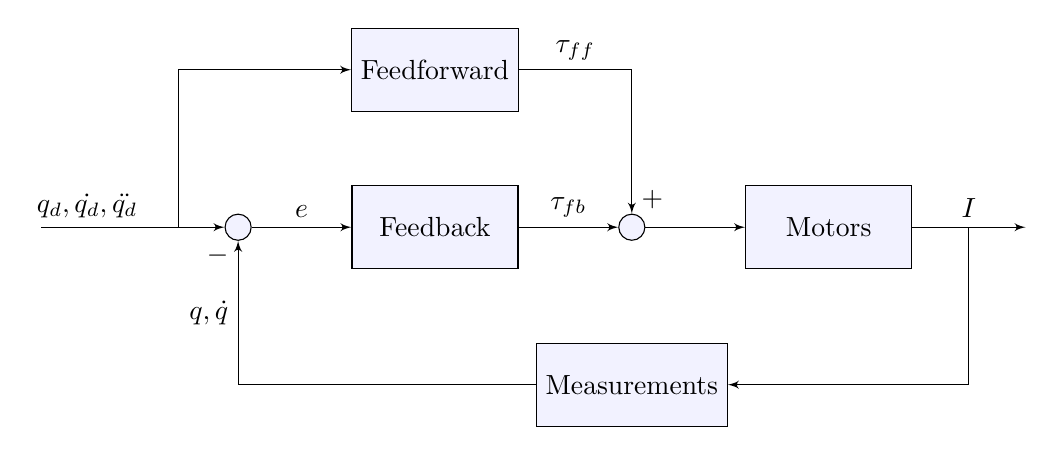
\begin{tikzpicture}[auto,node distance=2.5cm,>=latex']
% placing nodes
\node [input](input){};
\node [sum, right of=input](sum1){};
\node [block, right of=sum1](feedback){Feedback};
\node [block, above of=feedback, node distance=2cm](feedforward){Feedforward};
\node [sum, right of=feedback](sum2){};
\node [block, right of=sum2](motors){Motors};
\node [output, right of=motors](output){};
\node [block, below of=sum2, node distance=2cm](measurements){Measurements};
% connecting nodes
\draw [->](input) -- node[near start]{$q_d,\dot{q_d},\ddot{q_d}$} node[name=in,near end,below]{}(sum1);
\draw [->](in) |- (feedforward);
\draw [->](feedforward) -| node[near start]{$\tau_{ff}$} node[pos=0.95]{$+$}(sum2);
\draw [->](sum1) -- node{$e$} (feedback);
\draw [->](feedback) -- node{$\tau_{fb}$}(sum2);
\draw [->](sum2) -- (motors);
\draw [->](motors) -- node[name=I]{$I$}(output);
\draw [->](I) |- (measurements);
\draw [->](measurements) -| node[pos=0.95]{$-$} node[near end]{$q,\dot{q}$}(sum1); 
\end{tikzpicture}
\caption[Control scheme for Computed Torque controller.]{Control scheme for Computed Torque controller. $I$ is the vector of output current measured from joint actuators which is then transduced to joint positions and velocity.}
\label{fig:computedtorque}
\end{figure}

%%%%%%%%%%%%%%%%%%%%%%%%%%%%%%%%%%%%%%%%%%%%%%%%%%%%%%%%
\paragraph{Inverse Kinematics-based Controller}
Given an end-effector position and orientation, the problem of inverse kinematics consists in determining the corresponding joint configurations. Since the system to solve is in general nonlinear, it's not possible to compute a solution in closed-form. This leads to different scenarios, i.e.\ no admissible solutions in presence of structure singularities, multiple or infinite solutions if the robot is redundant (which is the case of KUKA LWR IV, see Section \ref{sec:therobot}). As an extension of the forward and inverse kinematics problem, it is also possible to define a relationship between the end-effector linear and angular velocity and the joint velocities as follows
\begin{equation}
\dot{x} = J\dot{q} \hspace{1cm} q \in \mathbb{R}^n,\,x \in \mathbb{R}^m
\label{eq:diffkinematics}
\end{equation}
representing the \textit{Differential Kinematics} equation. The mapping is described by the \textit{Jacobian} matrix $J \in \mathbb{R}^{m \times n}$ which depends on the robot configuration. Inverting \eqref{eq:diffkinematics}, leads to the \textit{Inverse Differential Kinematics} problem
\begin{equation}
\dot{q} = J^+\dot{x}
\end{equation}
where $J^+$ is a generalized inverse of the Jacobian. For the project's purpose, it has been implemented in ROS as the Moore-Penrose damped pseudo-inverse through the SVD method, denoted in the sequel as $J^{\dagger}$.\\
In view of the operational space formulation, given a desired end-effector pose $x_d$ and velocity $\dot{x}_d$, a task can be defined as 
\begin{equation}
e = x_d - x(t)
\end{equation}
where $x(t)$ is the end-effector pose at time t.
The related reference motion in the task space is
\begin{equation}
\dot{e}^* = \dot{x}_d + K(x_d - x) = \dot{x}_d + Ke
\end{equation}
where $K$ is a positive definite gain matrix (usually diagonal).

\begin{figure}[h]
\centering
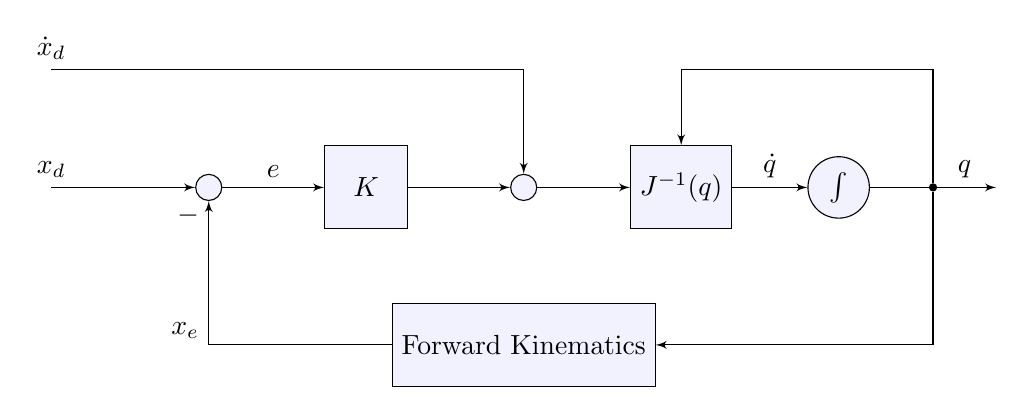
\begin{tikzpicture}[auto,node distance=2cm,>=latex']
% placing nodes
\node [input](input1){};
\node [input, above of=input1, node distance=1.5cm](input2){};
\node [sum, right of=input1](sum1){};
\node [block_small, right of=sum1](K){$K$};
\node [sum, right of=K](sum2){};
\node [block_small, right of=sum2](jac_inv){$J^{-1}(q)$};
\node [sum, right of=jac_inv](integral){$\int$};
\node [output, right of=integral](output){};
\node [block, below of=sum2](forw_kin){Forward Kinematics};
\coordinate [above of=integral,node distance=1.5cm](tmp);
%% connecting nodes
\draw [->](input1) -- node[pos=0]{$x_d$} (sum1);
\draw [->](input2) -| node[pos=0]{$\dot{x}_d$} (sum2);
\draw [->](sum1) -- node{$e$} (K);
\draw [->](K) -- (sum2);
\draw [->](sum2) -- (jac_inv);
\draw [->](jac_inv) -- node{$\dot{q}$} (integral);
\draw [->](integral) -- node[intersection,anchor=base,name=q]{} 
		   node[near end]{$q$} (output);
\draw [->](q) |- (tmp) -| (jac_inv);
\draw [->](q) |- (forw_kin);
\draw [->](forw_kin) -|  node[pos=0.55]{$x_e$} node[pos=0.95]{$-$} (sum1); 
\end{tikzpicture}

\caption{Control scheme for Differential Inverse Kinematics-based controller.}
\label{fig:diffinversekinematics}
\end{figure}

%%%%%%%%%%%%%%%%%%%%%%%%%%%%%%%%%%%%%%%%%%%%%%%%%%%%%%%%
\paragraph{Hierarchical Inverse Kinematics Controller}
It is possible to exploit the redundancy of the manipulator, i.e.\ when the rank of $J$ is smaller than $n$, to assign a secondary task by projecting an arbitrary vector on the null-space of the Jacobian, thus not affecting the higher priority task. So, considering two tasks $e_1$ and $e_2$, the following control law will perform exactly $\dot{e}_1^*$ and, if possible, $\dot{e}_2^*$
\begin{equation}
\dot{q} = J_1^{\dagger}\dot{e}_1^* + (J_{2}P_1)^{\dagger}(\dot{e}_2^* - J_{2}J_1^{\dagger}\dot{e}_1^*)
\end{equation}
This method is called \textit{Stack of Tasks} and can be generalized for $k$ tasks, ensuring a correct hierarchy between them \cite{mansardICAR09},\cite{mansardIEEE09}
\begin{equation}
\begin{dcases}
\dot{q}_0 = 0\\
P_0 = I_n\\
\dot{q}_i = \dot{q}_{i-1} + (J_{i}P_{i-1})^{\dagger}(\dot{e}_i^* - J_{i}\dot{q}_{i-1})\\
P_i = P_{i-1} + (J_{i}P_{i-1})^{\dagger}(J_{i}P_{i-1})
\end{dcases}
\end{equation}
where $P_i$ is the projection operator onto the null-space of $J_i$ and the robot joint velocity realizing all the tasks is $\dot{q}=\dot{q}_k$. This way, all the tasks are decoupled from each other and if a task won't be feasible it will be executed only at its best without disturbing the higher priority tasks.

\begin{figure}
\centering
\includegraphics[width=0.9\textwidth]{hik}
\caption{Simulated robot performing two tasks at different priority levels using Hierarchical Inverse Kinematics.}
\end{figure}

\begin{figure}
\centering
\includegraphics[width=\textwidth]{invkin}
\caption{Evolution of the Mean Square Error (MSE) of two tasks controlled through Hierarchical Inverse Kinematics.}
\end{figure}

%%%%%%%%%%%%%%%%%%%%%%%%%%%%%%%%%%%%%%%%%%%%%%%%%%%%%%%%
\paragraph{Inverse Dynamics-based Controller}
The problem of inverse dynamics in the operational space consists in the determination of the joint torques $\tau$ that realizes a specific motion $\ddot{e}^*$ assigned in terms of $\ddot{x}_d,\dot{x}_d,x_d$, the end-effector desired acceleration,velocity and position
\begin{equation}
\ddot{e}^* = \ddot{x}_d + K_d(\dot{x}_d - \dot{x}) + K_p(x_d - x) = 
\ddot{x}_d + K_{d}\dot{e} + K_{p}e
\end{equation}
where $K_p$ and $K_d$ are positive definite diagonal matrices. Recalling the manipulator dynamic model in the compact form \eqref{eq:compactrobotdynamics}, the choice of the \textit{inverse dynamics control}
\begin{equation}
\tau = M(q)y + n(q,\dot{q})
\end{equation}
leads to a double integrators system
\begin{equation*}
\ddot{q} = y
\end{equation*}
where the control $y$ is designed to track the desired motion $\ddot{e}^*$ through the following second-order relationship
\begin{equation}
\ddot{e}^* = J(q)\ddot{q} + \dot{J}(q,\dot{q})\dot{q}
\end{equation}
It is then possible to write, omitting dependencies in $q$ and its derivatives
\begin{equation}
\ddot{e}^* + b = JM^{-1}\tau
\label{eq:tempinvdyn}
\end{equation}
where $b = JM^{-1}n - \dot{J}(q,\dot{q})\dot{q}$.
Defining $\Omega = JM^{-1}J^T$ and $\Lambda = \Omega^{-1}$ and multiplying \eqref{eq:tempinvdyn} by $\Lambda$ leads to
\begin{equation}
\Lambda\ddot{e}^* + {\Lambda}b = \bar{J}^T\tau
\label{eq:temp2invdyn}
\end{equation}
where $\bar{J} = M^{-1}J^T\Lambda$ is the generalized inverse of $J$ weighted by $M^{-1}$. Finally, multiplying \eqref{eq:temp2invdyn} by $J^T$ it is possible to define the control law that realizes the reference motion $\ddot{e}^*$
\begin{equation}
\tau = J^T\Lambda(\ddot{e}^* + b)
\label{eq:onetaskinversedynamics}
\end{equation}

%%%%%%%%%%%%%%%%%%%%%%%%%%%%%%%%%%%%%%%%%%%%55
\paragraph{Hierarchical Inverse Dynamics Controller}
Equation \eqref{eq:onetaskinversedynamics} implements the inverse dynamics control for a single task $e$. As for inverse kinematics, the manipulator redundancy can be exploited also at dynamics level to give the possibility to execute other lower priority tasks, using the \textit{Stack of Tasks} framework (applied to $k$ tasks)
\begin{equation}
\begin{dcases}
\tau_0 = 0\\
{N_0}^T = I_n\\
\tau_i = \tau_{i-1} + {J_i}^T\Lambda_{i\vert i-1}({\ddot{e}_i}^* + b_i - J_{i}M^{-1}\tau_{i-1}) \\
{N_i}^T = {N_{i-1}}^T - {J_i}^T\Lambda_{i\vert i-1}J_{i}M^{-1}
\end{dcases}
\end{equation}
where $\Lambda_{i\vert i-1} = {\Omega_{i\vert i-1}}^{-1}$ and ${\Omega_{i\vert i-1}} = {J_i}^{T}M^{-1}{N_{i-1}}^TJ_i$. The projection operator is ${N_i}^T$ and the control $\tau$ applied to the robot is $\tau_k$.

\begin{figure}
\centering
\includegraphics[width=0.9\textwidth]{hid}
\caption{Simulated robot performing two tasks at different priority levels using Hierarchical Inverse Dynamics.}
\end{figure}

\begin{figure}
\centering
\includegraphics[width=0.9\textwidth]{invdyn}
\caption[Evolution of the Mean Square Error (MSE) of two tasks controlled through Hierarchical Inverse Dynamics.]{Evolution of the Mean Square Error (MSE) of two tasks controlled through Hierarchical Inverse Dynamics. Notice in the zoomed plot how the higher priority task converges to zero faster.}
\end{figure}

%%%%%%%%%%%%%%%%%%%%%%%%%%%%%%%%%%%%%%%%%%%%%%%%%%%%%%%%%%%%%%%%%%%
\paragraph{Minimum Effort Controller}
Another way to take advantage of the redundant DOFs, other than performing additional motion tasks, is to use the Jacobian null-space projection method to maximize an objective function in the joint space as follows
\begin{equation}
\tau = J^T\Lambda(\ddot{e}^* + b) + N^T\tau_{null}
\label{eq:projectednullspaceobjective}
\end{equation}
where in general $\tau_{null} = \nabla_{q}H(q)$ and $H(q)$ is a differentiable objective funcion to be maximized, implementing a specific criterion with the goal of moving the manipulator in its gradient direction. Taking inspiration from human manipulation, it is possible to reproduce those natural motions in an efficient way, setting the objective function $H(q) = g(q)^{T}Wg(q)$, where $g(q)$ is the gravitational force vector as in \eqref{eq:robotdynamics} and $W$ is a constant diagonal weighting matrix \cite{ajoudani13}. This way, control law \eqref{eq:projectednullspaceobjective} will minimize joint masses and payload gravitational forces while guaranteeing asymptotic stability of the system and not affecting the primary motion task referenced by $\ddot{e}^*$.

\begin{figure}
\centering
\includegraphics[width=0.9\textwidth]{minimumeffort_rviz}
\caption{Simulated robot tracking a circle figure using the Minimum Effort Controller.}
\end{figure}

\begin{figure}
	\centering
	\begin{subfigure}[t]{0.9\textwidth}
		\includegraphics[width=\textwidth]{minimumeffort_X}
		\subcaption{X-Axis}
	\end{subfigure}
	\begin{subfigure}[t]{0.9\textwidth}
		\includegraphics[width=\textwidth]{minimumeffort_Y}
		\subcaption{Y-Axis}
	\end{subfigure}
	\begin{subfigure}[t]{0.9\textwidth}
		\includegraphics[width=\textwidth]{minimumeffort_Z}
		\subcaption{Z-Axis}
	\end{subfigure}
	\caption{Axis-specific end-effector trajectories tracking a circle figure using Minimum Effort Control.}
\end{figure}

%%%%%%%%%%%%%%%%%%%%%%%%%%%%%%%%%%%%%%%%%%%%%%%%%%%%%%%%
\paragraph{Backstep Controller}
Backstepping is a recursive methodology for designing both feedback control laws and associated Lyapunov functions in a systematic way, with the goal of obtaining a good flexibility over the nonlinearities. Consider the following nonlinear system in which the origin is an equilibrium
\begin{equation}
\begin{dcases}
\dot{\xi}_1 = f(\xi_1) + g(\xi_1)\xi_2 \\
\dot{\xi}_2 = h(\xi_1,\xi_2) + \ell(\xi_1,\xi_2)u
\end{dcases}
\label{eq:backsteppingsystem}
\end{equation}
with $\xi_1\in\mathbb{R}^{n_1}, \xi_2\in\mathbb{R}^{n_2},u\in\mathbb{R}^{n_2}$ and $\ell(\xi_1,\xi_2)\in\mathbb{R}^{n_2 \times n_2}$ is invertible for all $\xi_1,\xi_2$. Assume that a stabilizing feedback law $u'=\Gamma(\xi_1)$ exists for the subsystem 
\begin{equation}
\dot{\xi}_1 = f(\xi_1) + g(\xi_1)u'
\end{equation}
and that a Lyapunov function $V(\xi_1)$ is postulated such that
\begin{equation}
\dot{V}(\xi_1) = V_{\xi_1}(f + g\Gamma)
\end{equation}
is at least negative semi-definite, with $V_{\xi_1} = \frac{\partial{V}}{\partial{\xi_1}}$. So, the control of the whole system \eqref{eq:backsteppingsystem} is obtained making $\xi_2$ to track the value of $u'=\Gamma(\xi_1)$.

\begin{figure}[H]
	\centering
	\includegraphics[width=0.9\textwidth]{backstepping_rviz}
	\caption{Simulated robot tracking a 8 figure using Backstepping Control.}
\end{figure}

The backstepping control method can be applied to a robotic manipulator described by its dynamic model \eqref{eq:robotdynamics}, designing the joint torques $\tau$ that track the trajectory $q_d(t)$. Defining the tracking error $e=q-q_d$ and its derivative $\dot{e}=w$, it is possible to consider the following system
\begin{equation}
\begin{dcases}
\dot{e} = w\\
\dot{w} = \ddot{q}-\ddot{q}_d = -\ddot{q}_d - M^{-1}\left(C\dot{q}+g(q)\right) + M^{-1}\tau
\end{dcases}
\label{eq:lagrangianbackstepping}
\end{equation}
which can be interpreted in the form of \eqref{eq:backsteppingsystem}, imposing $e=\xi_1, w=\xi_2, f(e)=0, g(e)=1, \ell(e,t)=M(e+q_d)^{-1}$ and $h(e,w,t)=-\ddot{q}_d(t)-M^{-1}\left(C(\dot{e}+\dot{q}_d)+g\right)$. After performing a stability study with Lyapunov control functions, the backstepping control law for a fully actuated manipulator can be defined as
\begin{equation}
\tau = M\ddot{q}_r + C\dot{q}_r + g(q) - K_{d}s - e
\label{eq:backsteppingcontrollaw}
\end{equation}
where
\begin{align*}
s &= \dot{e} + \Lambda{e}\\
&= \dot{q} - (\dot{q}_d - \Lambda{e}) = \dot{q} - \dot{q}_r
\end{align*}
and $\dot{q}_r$ is the so-called reference velocity. 

\begin{figure}
	\centering
	\begin{subfigure}[t]{0.9\textwidth}
		\centering
		\includegraphics[width=\textwidth]{backstepping_X}
		\subcaption{X-Axis}
	\end{subfigure}
	\begin{subfigure}[t]{0.9\textwidth}
		\centering
		\includegraphics[width=\textwidth]{backstepping_Y}
		\subcaption{Y-Axis}
	\end{subfigure}
	\begin{subfigure}[t]{0.9\textwidth}
		\centering
		\includegraphics[width=\textwidth]{backstepping_Z}
		\subcaption{Z-Axis}
	\end{subfigure}
	\caption{Axis-specific end-effector trajectories tracking a 8 figure using Backstepping Control.}
\end{figure}

%%%%%%%%%%%%%%%%%%%%%%%%%%%%%%%%%%%%%%%%%%%%%%%%%%%%%%%%
\paragraph{Dynamic Sliding PID Controller}
Regarding simple tasks such as set-point regulation, a proportional-integral-derivative (PID) controller would be enough, but the limitation of this class of controllers is that they can't achieve asymptotic stability for trajectory tracking. However, it is possible to enhance PID controllers by applying to them the sliding mode theory, as explained in the sequel \cite{parravega03}. So, given a desired motion specified by $q_d,\dot{q}_d,\ddot{q}_d\in\mathbb{R}^n$, it is analyzed the problem of designing the controller $\tau$ which guarantees the tracking of $q_d(t)$ without any knowledge of the system dynamic model and without introducing high-frequency components, by considering the following steps
\begin{align}
&\dot{q}_r = \dot{q}_d - \alpha\Delta{q} + S_d - \gamma\sigma \label{eq:sliding_qdotref}\\
&\dot{\sigma} = sgn(S_q)
\end{align}
where $\Delta{q}$ is the tracking error $q-q_d$, $\alpha,\gamma\in\mathbb{R}^{n \times n}$ are diagonal positive definite gain matrices and $sgn(S_q)$ represents the input-wise discontinuous signum function of $S_q\in\mathbb{R}^n$, the so-called sliding surface, being defined by
\begin{align}
&S_q = S - S_d\\
&S = \Delta{\dot{q}} + \alpha\Delta{q}\\
&S_d = S(t_0)e^{-\kappa(t-t_0)}
\end{align}
with $\kappa > 0$.
Considering a new error coordinates $S_r$ defined as
\begin{equation}
S_r = \dot{q} - \dot{q}_r
\end{equation}
and substituting $\dot{q}_r$ as in \eqref{eq:sliding_qdotref}, it leads to
\begin{equation}
S_r = S_q + \gamma\sigma
\end{equation}
Finally, the controller $\tau$ which realizes the tracking of $q_d(t)$ in closed loop is
\begin{equation}
\tau = -K_{d}S_r
\end{equation}
where $K_d\in\mathbb{R}^{n \times n}$ is a diagonal symmetric positive definite matrix. According to the controller structure, the semi-global exponential tracking is assured and the passivity of the system is preserved, as long as $\gamma$ in \eqref{eq:sliding_qdotref} and $K_d$ are large enough, for small initial conditions.

\begin{figure}[H]
	\centering
	\begin{subfigure}[t]{0.9\textwidth}
		\centering
		\includegraphics[width=\textwidth]{slidingmode_j1}
		\subcaption{Joint 1}
	\end{subfigure}
	\begin{subfigure}[t]{0.9\textwidth}
		\centering
		\includegraphics[width=\textwidth]{slidingmode_j3}
		\subcaption{Joint 3}
	\end{subfigure}
	\caption{Joint-specific sine waves trajectories tracking using Dynamic Sliding PID Control.}
\end{figure}

\subsubsection{Joint state estimation}

One issue found during the implementation of controllers is the absence of joint velocity values. While the simulated hardware interface takes the joint velocity from simulation, the KUKA LWR arm is equipped with position and torque sensors. Thus, the need to derive the velocities from the position values through a process of online differentiation is prominent. The following methods were visited.

\paragraph{Levant Robust Differentiator}
This method is based on the sliding mode theory and gives asymptotically exact derivatives~\cite{levant06}. In comparison with the Euler method, Levant differentiator performs significantly better in terms of noise rejection and derivation of signals, but the major flaw which led this method to be discarded is that introduces a relevant phase shift. 
\paragraph{Euler method}
This is one of the most basic techniques to compute numerical differentiation and follows the equation
\begin{equation}
\dot{q}_n = \frac{q_n - q_{n-1}}{h},
\end{equation}
where $h$ is the sampling time. Since the output of this differentiator is usually noisy, typically, a exponential smoothing filter is used as the post-process signal processing as
\begin{equation}
\tilde{\dot{q}}_n = \alpha\dot{q}_n + (1-\alpha)\tilde{\dot{q}}_{n-1},
\end{equation}
where $\tilde{\dot{q}}$ denotes the smoothed value and $\alpha\in(0,1)$ is the smoothing factor. This is the current joint state estimation method for the arm.
%So, according to the tests conducted and evaluating a trade-off between exact but out-of-phase signals and noisy but coherent signals, the best method resulted the Euler one.

% %%%%%%%%%%%%%%%%%%%%%%%%%%%%%%%%%%%%%%%%%%%%%%%%%%%%%%%%
% %%%%%%%%%%%%%%%%%%%%%%%%%%%%%%%%%%%%%%%%%%%%%%%%%%%%%%%%
% %%%%%%%%%%%%%%%%%%%%%%%%%%%%%%%%%%%%%%%%%%%%%%%%%%%%%%%%
% \subsubsection{Controller design issues}
% During the process of controllers design, certainly one requirement that has to be met is to reach an efficient complexity in terms of computational resources. In the sequel it's analyzed a category of control strategies which requires, at least in this case study, the exploitation of a big amount of resources that unfortunately weren't available on the machines used for experiments.

% %%%%%%%%%%%%%%%%%%%%%%%%%%%%%%%%%%%%%%%%%%%%
% \paragraph{Adaptive Control}
% In this section it has been assumed that the dynamic model of the robot is perfectly known at any instant of time, but, in practice, this can't be always true. In fact there exist some model uncertainties depending on the robot configuration, mainly mechanical parameters like inertia matrices and masses for the single links or those related to the robot payload. To overcome this intrinsic problem, it is always possible to write the dynamic model of the robot \eqref{eq:robotdynamics} through a linear parametrization
% \begin{equation}
% M(q)\ddot{q} + C(q,\dot{q})\dot{q} + g(q) = Y(q,\dot{q},\ddot{q})\pi = \tau
% \end{equation}
% where the vector $\pi\in\mathbb{R}^r$ contains the combinations of the aforementioned physical parameters and $Y(q,\dot{q},\ddot{q})\in\mathbb{R}^{n\times r}$ is called the \textit{regressor} matrix. In brief, this sums up the aim of the \textit{Adaptive Control}, which, as the name suggests, makes the control law to adapt to the variations of the unknown robot model parameters. Recently, an analytic closed formula for the regressor has been derived from the Lagrange equations, in terms of the Denavit-Hartenberg parameters and the joints configurations  $q,\dot{q},\ddot{q}$, and implemented in \textit{Mathematica} environment \cite{gabiccini09}. For a 7-links manipulator like KUKA LWR, the resulting regressor matrix has dimensions $7$x$70$ in its unsimplified form, making literally impossible to handle an adaptive control with the owned instruments.

% %%%%%%%%%%%%%%%%%%%%%%%%%%%%%%%%%%%%%%%%%%%%
% \paragraph{Gravity Compensation}
% Recalling the built-in controllers \eqref{eq:cartesianstiffnesscontroller}, \eqref{eq:axisspecificstiffnesscontroller} of the KUKA LWR arm, the term $f_{dynamics}(q,\dot{q},\ddot{q})$ must be analyzed. It refers to the gravity compensation performed internally by the robot, in a way that the commanded torque isn't indeed affected by the gravitational field. This, unfortunately, generates a conflict between the internal compensation and the whole control law, which at dynamic level requires the knowledge of the gravitational force to compute the input torques. Since such term can't be forced to zero, one workaround could be that of not considering the gravity ($g(q)=0$) in all model-based controller, introducing a really negligible error.
%!TEX root = MS42.tex
\section{Software Environment}
\subsection{Robot Software Development}
The middleware software used to implement the robot software is \textit{Robot Operating System} (mostly known as ROS) \cite{webros}. Actually, ROS is not just an operating system, it's a complete ecosystem providing libraries, hardware abstraction, device drivers, visualizers, message-passing and package management. 

\subsubsection{How ROS Works}
Basically, the ROS system is based on nodes, topics, messages and services, allowing the developer to work on a simple and modular code structure.

\subparagraph*{Nodes}
\textit{Nodes} are processes that perform a specific task. They can use \textit{topics} to communicate between each other and use \textit{services} to handle external operations, e.g.\ a remote procedure call.

\subparagraph*{Topics}
\textit{Topics} are the transport system used to delivery \textit{messages} between \textit{nodes}. They are based on the \textit{publish/subscribe} semantics, so that a node sends out a message by publishing it on a specific topic. On the other hand, a node will subscribe to the appropriate topic to which it is interested.

\subparagraph*{Messages}
\textit{Messages} are simply structures of data of typed fields. Just like \textit{C}, they support both standard and user-defined types, as well as nested and complex structures.

\subparagraph*{Services}
The \textit{publish/subscribe} model, even being a flexible and strong communication system, can't afford the \textit{request/reply} interactions, which is managed by the \textit{services}. An example of usage could be a situation in which a node has executed a task and needs a feedback or an acknowledge for it.

\subsection{Simulation Environment}
During the process of building robot applications, it's clearly not convenient to perform code debug and tests on the real robot. Therefore, the developer needs a simulated environment in which the behaviour of the real robot can be emulated via software in an as precise as possible way, replicating model dynamics, joints and links properties, loads handling and so on. The simulation software used for this purpose is \textit{Gazebo} \cite{webgazebo}, which offers a strict interaction with ROS, providing a realistic rendering of the robot along with its real time ROS-controlled behavior. 

\begin{figure}[H]
\centering
\includegraphics[width=\textwidth]{gazebo} 
\caption{Gazebo Simulator with KUKA LWR IV robot}
\end{figure}


\subsubsection{How Gazebo Works}
To render the robot, the developer has to build a XML file describing all elements of the robot following a tree structure. This file is easily built using the robot focused DSL (\textit{Domain Specific Language}) named URDF (\textit{Unified Robot Description Format}). Gazebo has the task of parsing the URDF model and, through a publish/subscribe system with the ROS nodes and topics, it can apply the user-defined algorithms and control laws to the simulated robot.

\subsection{Additional Tools}
\subsubsection{RViz}
Another software to mention, used mainly in simulation but also during real experiments, is \textit{RViz}, which is a 3D visualization tool included in ROS. It has been useful not only to monitor the current robot configuration (joint states, pose, orientation) but it's also capable of plotting executed trajectories.

\subsubsection{Kinematics and Dynamics Library (KDL)}
A great and valid support in coding has been given by the \textit{Kinematics and Dynamics Library} (KDL), a software framework providing class libraries for robot modeling, as well as computation of forward and inverse chain kinematics and dynamics, motion specification and so on \cite{webkdl}.

\begin{figure}[H]
\centering
\includegraphics[width=\textwidth]{rviz} 
\caption{Visualization of the KUKA LWR IV robot in RViz}
\end{figure}


\newpage
\input{controllers}
%!TEX root = MS42.tex
\section{Hardware Interface}
%Another flaw encountered regards the process of switching from the simulation environment to the real robot interface. As expected, even if the robot has been modeled and rendered almost perfectly for the simulation purpose, it lacks some important aspects of its dynamics.
\subsection{From Simulation to Real Robot}
The purpose of the development of robotics applications in a simulated environment is exactly to test and debug the software produced before loading it on the physical robot. To make this passage smooth and seamless, it has been implemented a hardware interface layer which provides an abstraction of the robot components, as shown in \autoref{fig:rosgazebointeraction}.
\begin{figure}[H]
\centerline{\includegraphics[scale=0.6]{ros+gazebo}}
\caption[Scheme of the interaction between ROS and Gazebo.]{Scheme of the interaction between ROS and Gazebo, with particulars on simulated and real robot.}
\label{fig:rosgazebointeraction}
\end{figure}
\subsubsection{Sensors Measurements (Joint State Interface)}
The major problem during the implementation regards the presence of sensors for joint velocities measurements. In fact, while Gazebo provides them accurately through simulated sensors, the KUKA LWR arm is only equipped with position and torque sensors. This, indeed, arises the need to derive the velocities from the measured positions through a process of online differentiation, with the following methods being analyzed
\paragraph{Euler Method}
This is one of the most basic techniques to compute numerical differentiation and its formulation is
\begin{equation}
\dot{q}_n = \frac{q_n - q_{n-1}}{h}
\end{equation}
where $h$ is the sampling time. Since the output of this differentiator is usually a bit noisy, it's convenient to pass it through an exponential smoothing filter, which is basically a weighted average between the last computed velocity value and the previous one
\begin{equation}
\tilde{\dot{q}}_n = \alpha\dot{q}_n + (1-\alpha)\tilde{\dot{q}}_{n-1} 
\end{equation}
where $\tilde{\dot{q}}$ denotes the smoothed value and $\alpha\in(0,1)$ is the smoothing factor.
\paragraph{Levant Robust Differentiator}
This method is based on the sliding mode theory and gives asymptotically exact derivatives \cite{levant06}. In comparison with Euler, Levant differentiator performs significantly better in terms of noise rejection and derivation of signals, but the major flaw which led this method to be discarded is that introduces a relevant phase shift.\\[1em]
So, according to the tests conducted and evaluating a trade-off between exact but out-of-phase signals and noisy but coherent signals, the best method resulted the Euler one.
\newpage
%!TEX root = MS42.tex
\section{Conclusions and Future Works}
The present work had the aim of implementing an extended set of different classes of controllers for the robotic arm KUKA LWR IV, exploiting a flexible system which is rapidly growing in the field of robotics, including research and whole industrial processes. In fact, all the code produced could not only be accessed and used from users operating the same robot, but ideally from everyone who works with ROS, at least performing some minor edits to fit their needs. Thinking about future works starting from this project, it could be interesting the extension to a bimanual system in a human-like arms configuration. For example, taking advantage of the Stack of Tasks framework could be also provided obstacle and collision avoidance, making easier the interaction between the robot and humans or the handling of more complex operations. 
\newpage


\bibliographystyle{IEEEtran}
\bibliography{bibliography/bibliography}

\end{document}
